\section{Cerberus: BB Aware Batch Scheduler}
\label{Sec:Scheduler}

\begin{figure}[htp]
        \centering
        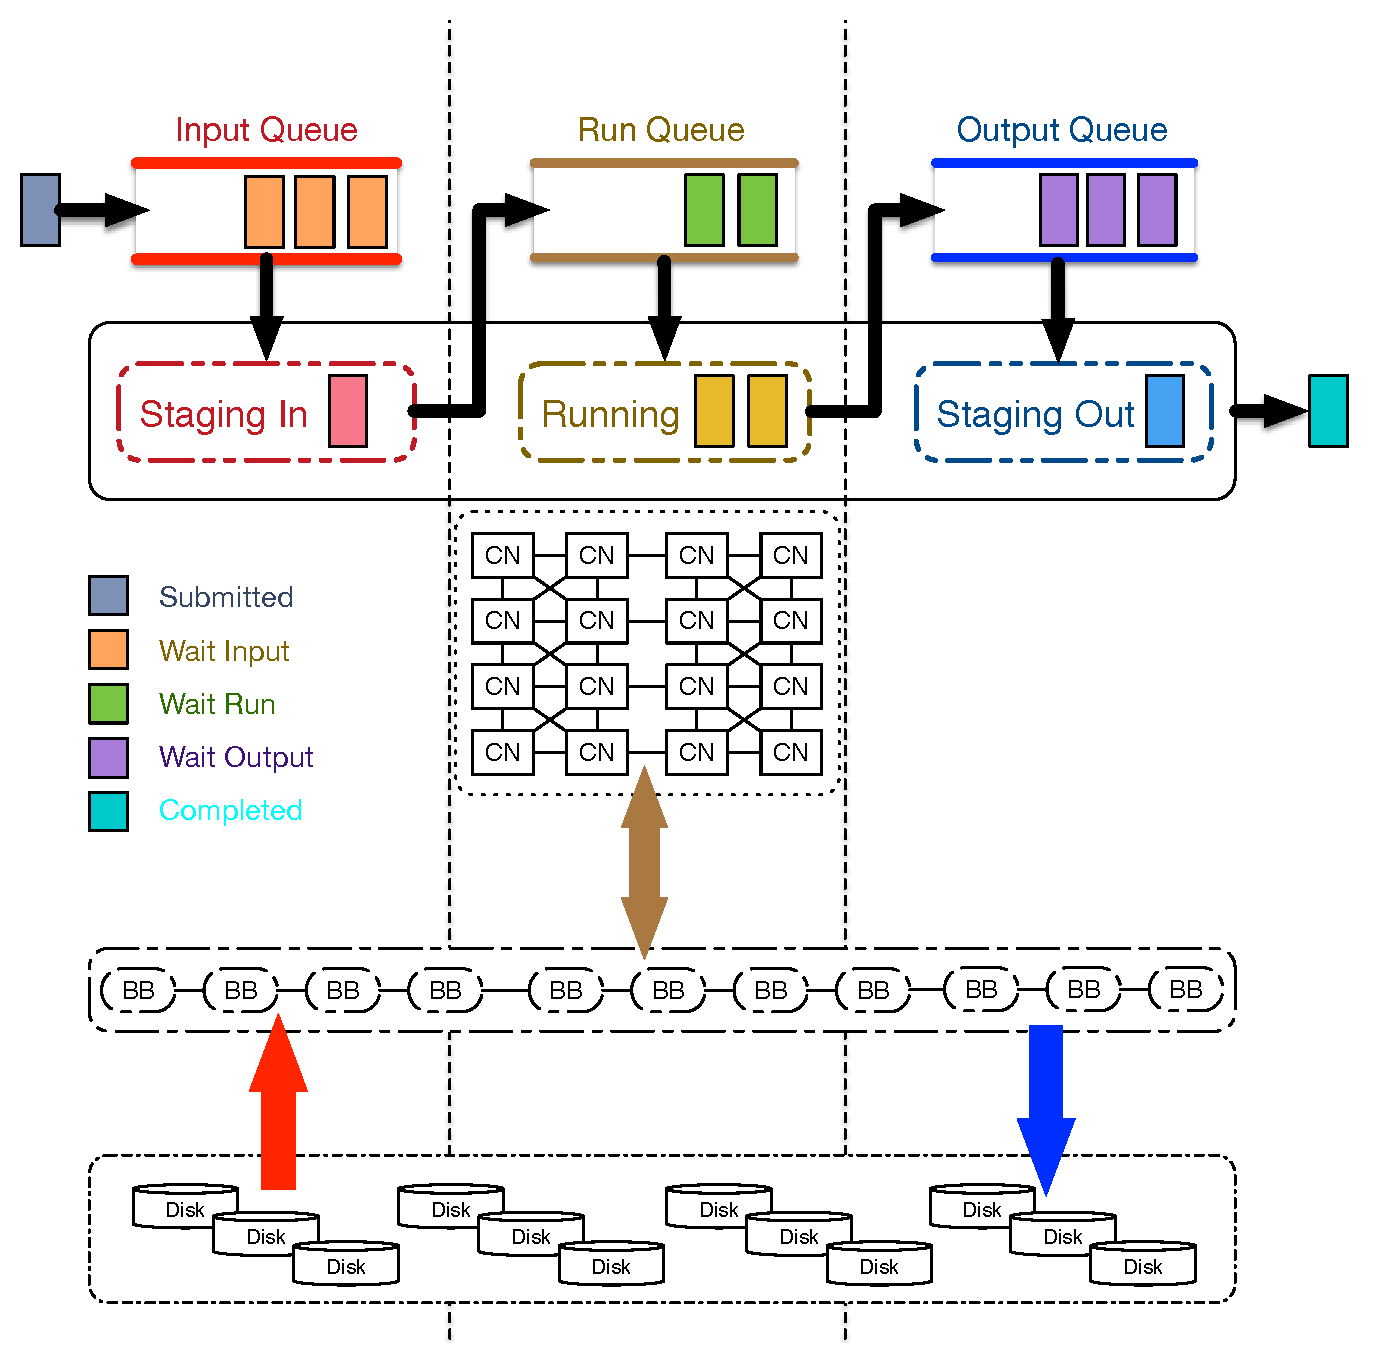
\includegraphics[width=3.6in]{CerberusBBSystem}
        \caption{Scheduling Workflow of Burst Buffer Aware Cerberus}
        \label{Fig:CerberusQueues}
\end{figure}

\begin{figure}[htp]
\centering
        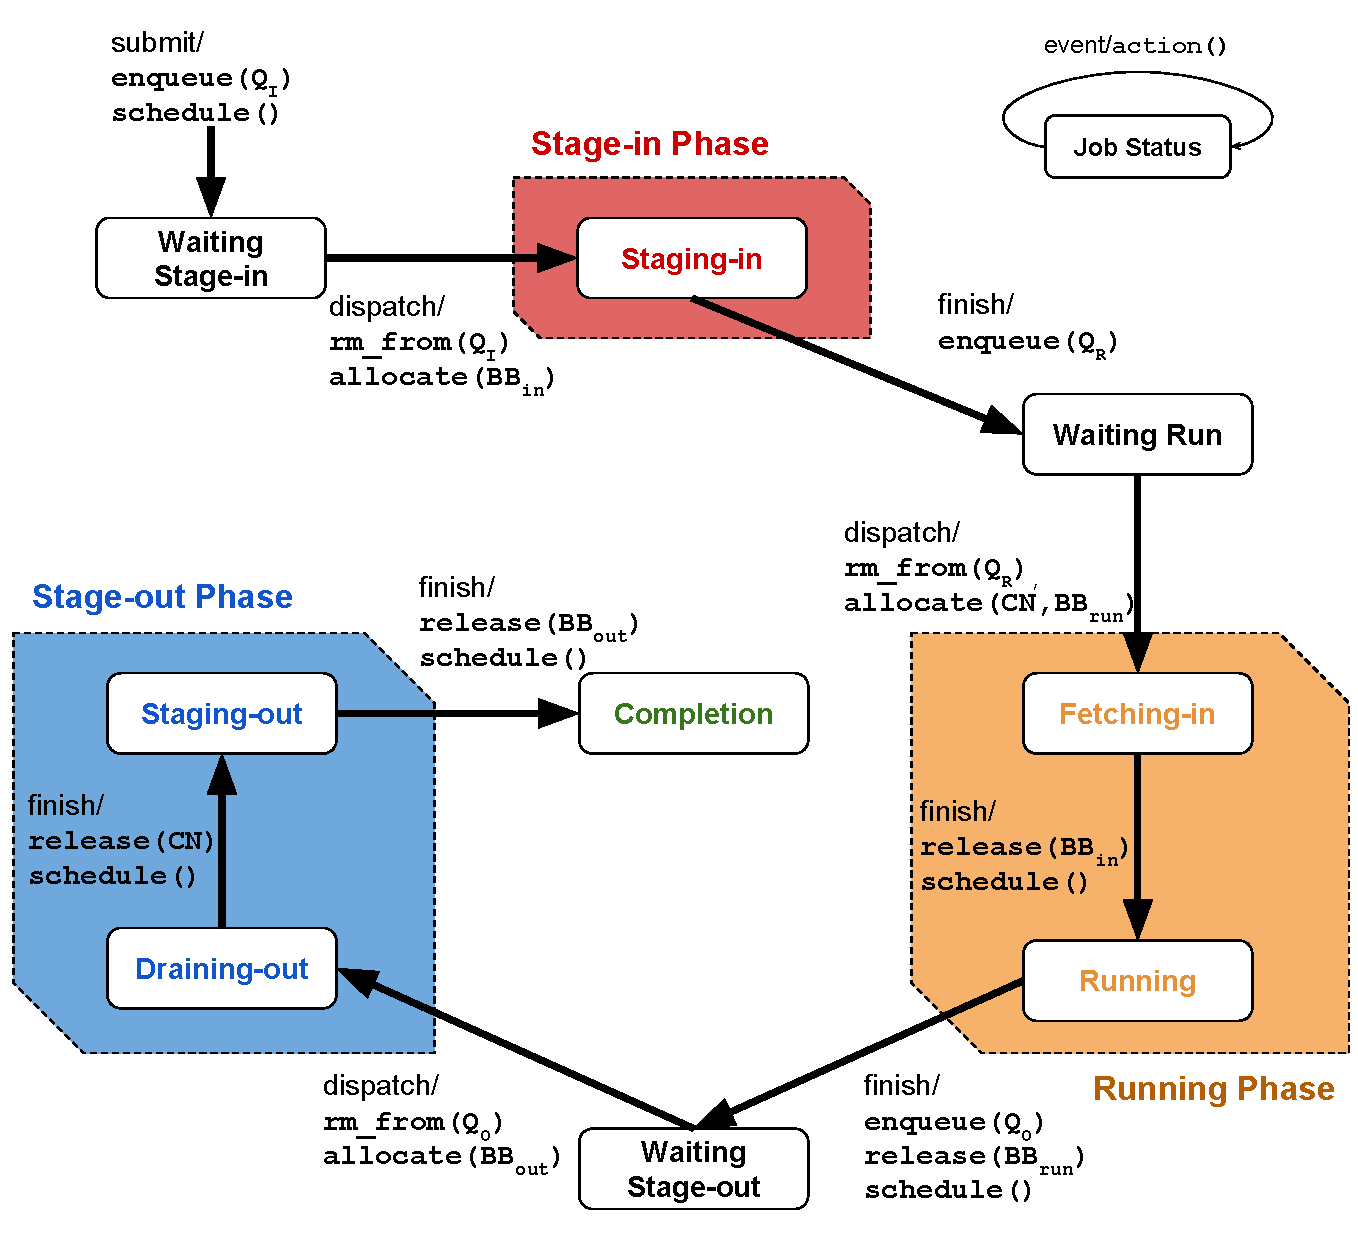
\includegraphics[width=3.6in]{3PhaseJobFSM}
        \caption{Event-driven BBsim scheduling model}
\label{Fig:JobFSM}
\end{figure}

\subsection{Scheduling Process}

The traditional batch scheduler on system without burst buffer only
takes job size (required number of nodes) and expected runtime into scheduling decision making. 
The most commonly used scheduling policy are First Come First Serve with
EASY backfilling~\cite{tsafrir-tpds-2007}.
However, on burst buffer enabled systems, 
the available amount of burst buffer capacity becomes a new scheduling constraint.
On the foundation of 3-phase job model,
we propose Cerberus, the batch scheduler with burst buffer awareness.
Cerberus is burst buffer aware because it fully takes the advantage of the 
most common usage cases of burst buffer: data stage-in, checkpointing, and data drain-out.
Burst buffer are allocated in each phase by Cerberus for one of the three usage.
This is done by maintaining 3 distinct queues, as shown in Figure~\ref{Fig:CerberusQueues},
Before entering each phase, job must enqueue to the corresponding queue.
The input queue $Q_I$ contains all the jobs that
needs to pre-fetch data from external storage to burst buffer.
The running queue $Q_R$ holds jobs
waiting for compute nodes and burst buffer used for checkpointing.
Jobs waiting to drain out output data to external permanent storage are in output queue $Q_O$.
The layered hierarchy in Figure~\ref{Fig:CerberusQueues} also indicates that
burst buffer fills in the memory gap between memory on compute nodes and disk storage.

To see how Cerberus schedules a particular job with 3 queues,
we have drawn a job's transition diagram in Figure~\ref{Fig:JobFSM}.
Upon submission, the job is enqueued into $Q_I$ to wait for stage-in-purpose burst buffer ($BB_{in}$).
When selected by Cerberus, job will be removed from $Q_I$ and
start to stage in data using allocated $BB_{in}$.
After finishing stage-in phase, the job is enqueued to $Q_R$, where it waits for
compute nodes and \textit{new} burst buffer specific for checkpointing ($BB_{run}$).
Notice that right now, $BB_{in}$ is still hold by this job.
At some time, Cerberus choose this job from $Q_R$.
Now the job is in running phase.
The first thing is to release $BB_{in}$ after fetching in data to memory on the acquired compute nodes.
During executing, checkpointing and application restart may happen frequently, which in essential
are data exchanges between memory and burst buffer $BB_{run}$.
Once job execution finishes, $BB_{run}$ can be immediately released since
output data are still available on the compute nodes.
Keeping holding these compute nodes, job enters $Q_O$ and waits for a certain amount of burst
buffer for staging out its data ($BB_{out}$).
Upon job being chosen by Cerberus, its data first flow from main memory to burst buffer
in the drain-out phase, after which all compute nodes can be released;
then burst buffer nodes is responsible for transfer output data to external storage system.
The lifetime of a job concludes when all useful data results are stored
and $BB_{out}$ are returned to system.
As indicated by Figure~\ref{Fig:JobFSM}, resource release at anytime will trigger Cerberus
scheduling jobs in possible multiple queues.

The 3-phase job model divides job to generic phases with specific resource demands.
Cerberus conquers the scheduling problem in each phase.
The finer scheduling granularity make it possible to fully utilize burst buffer for different purpose.
The consequential divide-conquer approach provides a framework that various scheduling
policy can be applied for each individual phase.
Both as demonstration of this framework and enhancement to Cerberus,
we propose and solve 2 optimizations targeting $Q_I/Q_O$ and $Q_R$ in Section~\ref{Sec:Opt}

\subsection{Coordination Among Three Phases}
The three phases of jobs, together with corresponding queues, are not entirely independent.
First, for a given job, its three phases are temporally dependent.
That is, only after finishing stage-in phase can a job be ready for running;
similarly, only when finishing running phase can a job waiting or entering stage-out phase.
This is reflected in the lifetime of a job's execution.

Secondly, for any job,
its burst buffer requested before entering a individual phase can only be used for a single purpose.
For example, a running-phase job cannot hold its already taken burst buffer
and use them to enter stage-out phase upon finishing running,
no matter whether holding burst buffer is enough to do so.
In Cerberus, resource release must be done mandatorily as specified in Figure~\ref{Fig:JobFSM},
We believe frequent release provides more opportunities to make
scheduler involve in each phase of scheduling the jobs.

At last, it is possible that all 3 queues are not empty at the moment of scheduling.
We choose a heuristic strategy to determine the scheduling order when
Cerberus has to handle multiple queues at the same time.
Noticing that jobs finishing \textit{running} and \textit{stage-out} phase
will fully or partially release taken resources,
we set the priority of queues to be $priority(Q_O) > priority(Q_R) > priority(Q_I)$.
This greedy heuristic works well when the demand of jobs in $J_{Q_I}$ is low.
However, it is possible to make jobs stacking up at the entry of the system.
We plan to investigate more on this problem in the future.


